\iffalse 

TODO : 
参考文献修正、フッターに書く?
リストのマークを変える、サイズ大きく
本文文字太くする?
画像があるといい

\fi

\RequirePackage{plautopatch} 
\documentclass[17pt,aspectratio=169]{beamer} 
\usepackage{amsmath}
\usepackage{amssymb}
\usepackage{graphicx}
\usepackage{luatexja}
\usepackage{luatexja-fontspec} 
\usepackage{fontspec}
\usepackage{color}
\usepackage{tcolorbox}
\usepackage{ascmac}
\usepackage{bm}
\usepackage{appendixnumberbeamer}
\usepackage{comment}

\usepackage{enumitem}
\setlist[itemize,1]{label=\textbullet, itemsep=17pt}  % 記号をもうちょっと大きくしたい
\setlist[itemize,2]{label=\textasteriskcentered, itemsep=3pt} 
\setlist[itemize,3]{label=\textendash, itemsep=3pt} 

\usetheme{metropolis}  % Metropolisテーマを使用
\setmainjfont{Yu Gothic Bold}  
\setsansjfont{Yu Gothic Bold}  

%Beamerフォント設定 
\usefonttheme{professionalfonts} % Be professional!
\usepackage[T1]{fontenc}
\usepackage{mlmodern}  % 太いComputer Modern
% MLmodernのバグを修正: cf. https://tex.stackexchange.com/questions/646333/size-of-integral-symbol-in-section-header-with-mlmodern
\DeclareFontFamily{OMX}{mlmex}{}
\DeclareFontShape{OMX}{mlmex}{m}{n}{%
   <->mlmex10%
   }{} 
\renewcommand{\familydefault}{\sfdefault}  % 英文をサンセリフ体に
\renewcommand{\kanjifamilydefault}{\gtdefault}  % 日本語をゴシック体に
\usefonttheme{structurebold} % タイトル部を太字
\setbeamerfont{alerted text}{series=\bfseries} % Alertを太字
\setbeamerfont{section in toc}{series=\mdseries} % 目次は太字にしない
\setbeamerfont{frametitle}{size=\large} % フレームタイトル文字サイズ
\setbeamerfont{title}{size=\LARGE} % タイトル文字サイズ
\setbeamerfont{date}{size=\normalsize}  % 日付文字サイズ
\setbeamerfont{author}{size=\normalsize}  % 日付文字サイズ
\setbeamerfont{normal text}{series=\mdseries} % 本文を太字に 

%ページ番号の設定
\setbeamertemplate{footline}{
    \hfill {\textcolor{gray!90}{\insertframenumber/\inserttotalframenumber}\hspace{0.1cm}}
    \vspace{0.1cm} 
}

%短縮形
\newcommand{\Pbb}{\mathbb{P}}
\newcommand{\Gcal}{\mathcal{G}}
\newcommand{\Fcal}{\mathcal{F}}

%タイトル
\title{¬ACの相対的無矛盾性証明のIsabelle/ZFによる形式化}
\author{東北大学 大学院情報科学研究科 住井・松田研究室 \\ 舟根大喜}
\date{October 14, 2024}

\begin{document}
\maketitle

\begin{frame}{概要}
    aaaa
%やったことと意義,背景
\end{frame}

\section{Isabelle/ZFについて}

\begin{frame}{定理証明支援系}
    \begin{columns}
        \begin{column}{0.65\textwidth}
            \begin{itemize}[itemsep=7pt]
                \item 数学的証明の形式化や、\\ソフトウェアの正しさの証明\\などに用いられるシステム
                \item プログラムを書くように\\定義・証明を記述する
                \item Isabelleはその一種
            \end{itemize}

        \end{column}
        \begin{column}{0.35\textwidth}
            \begin{figure}
                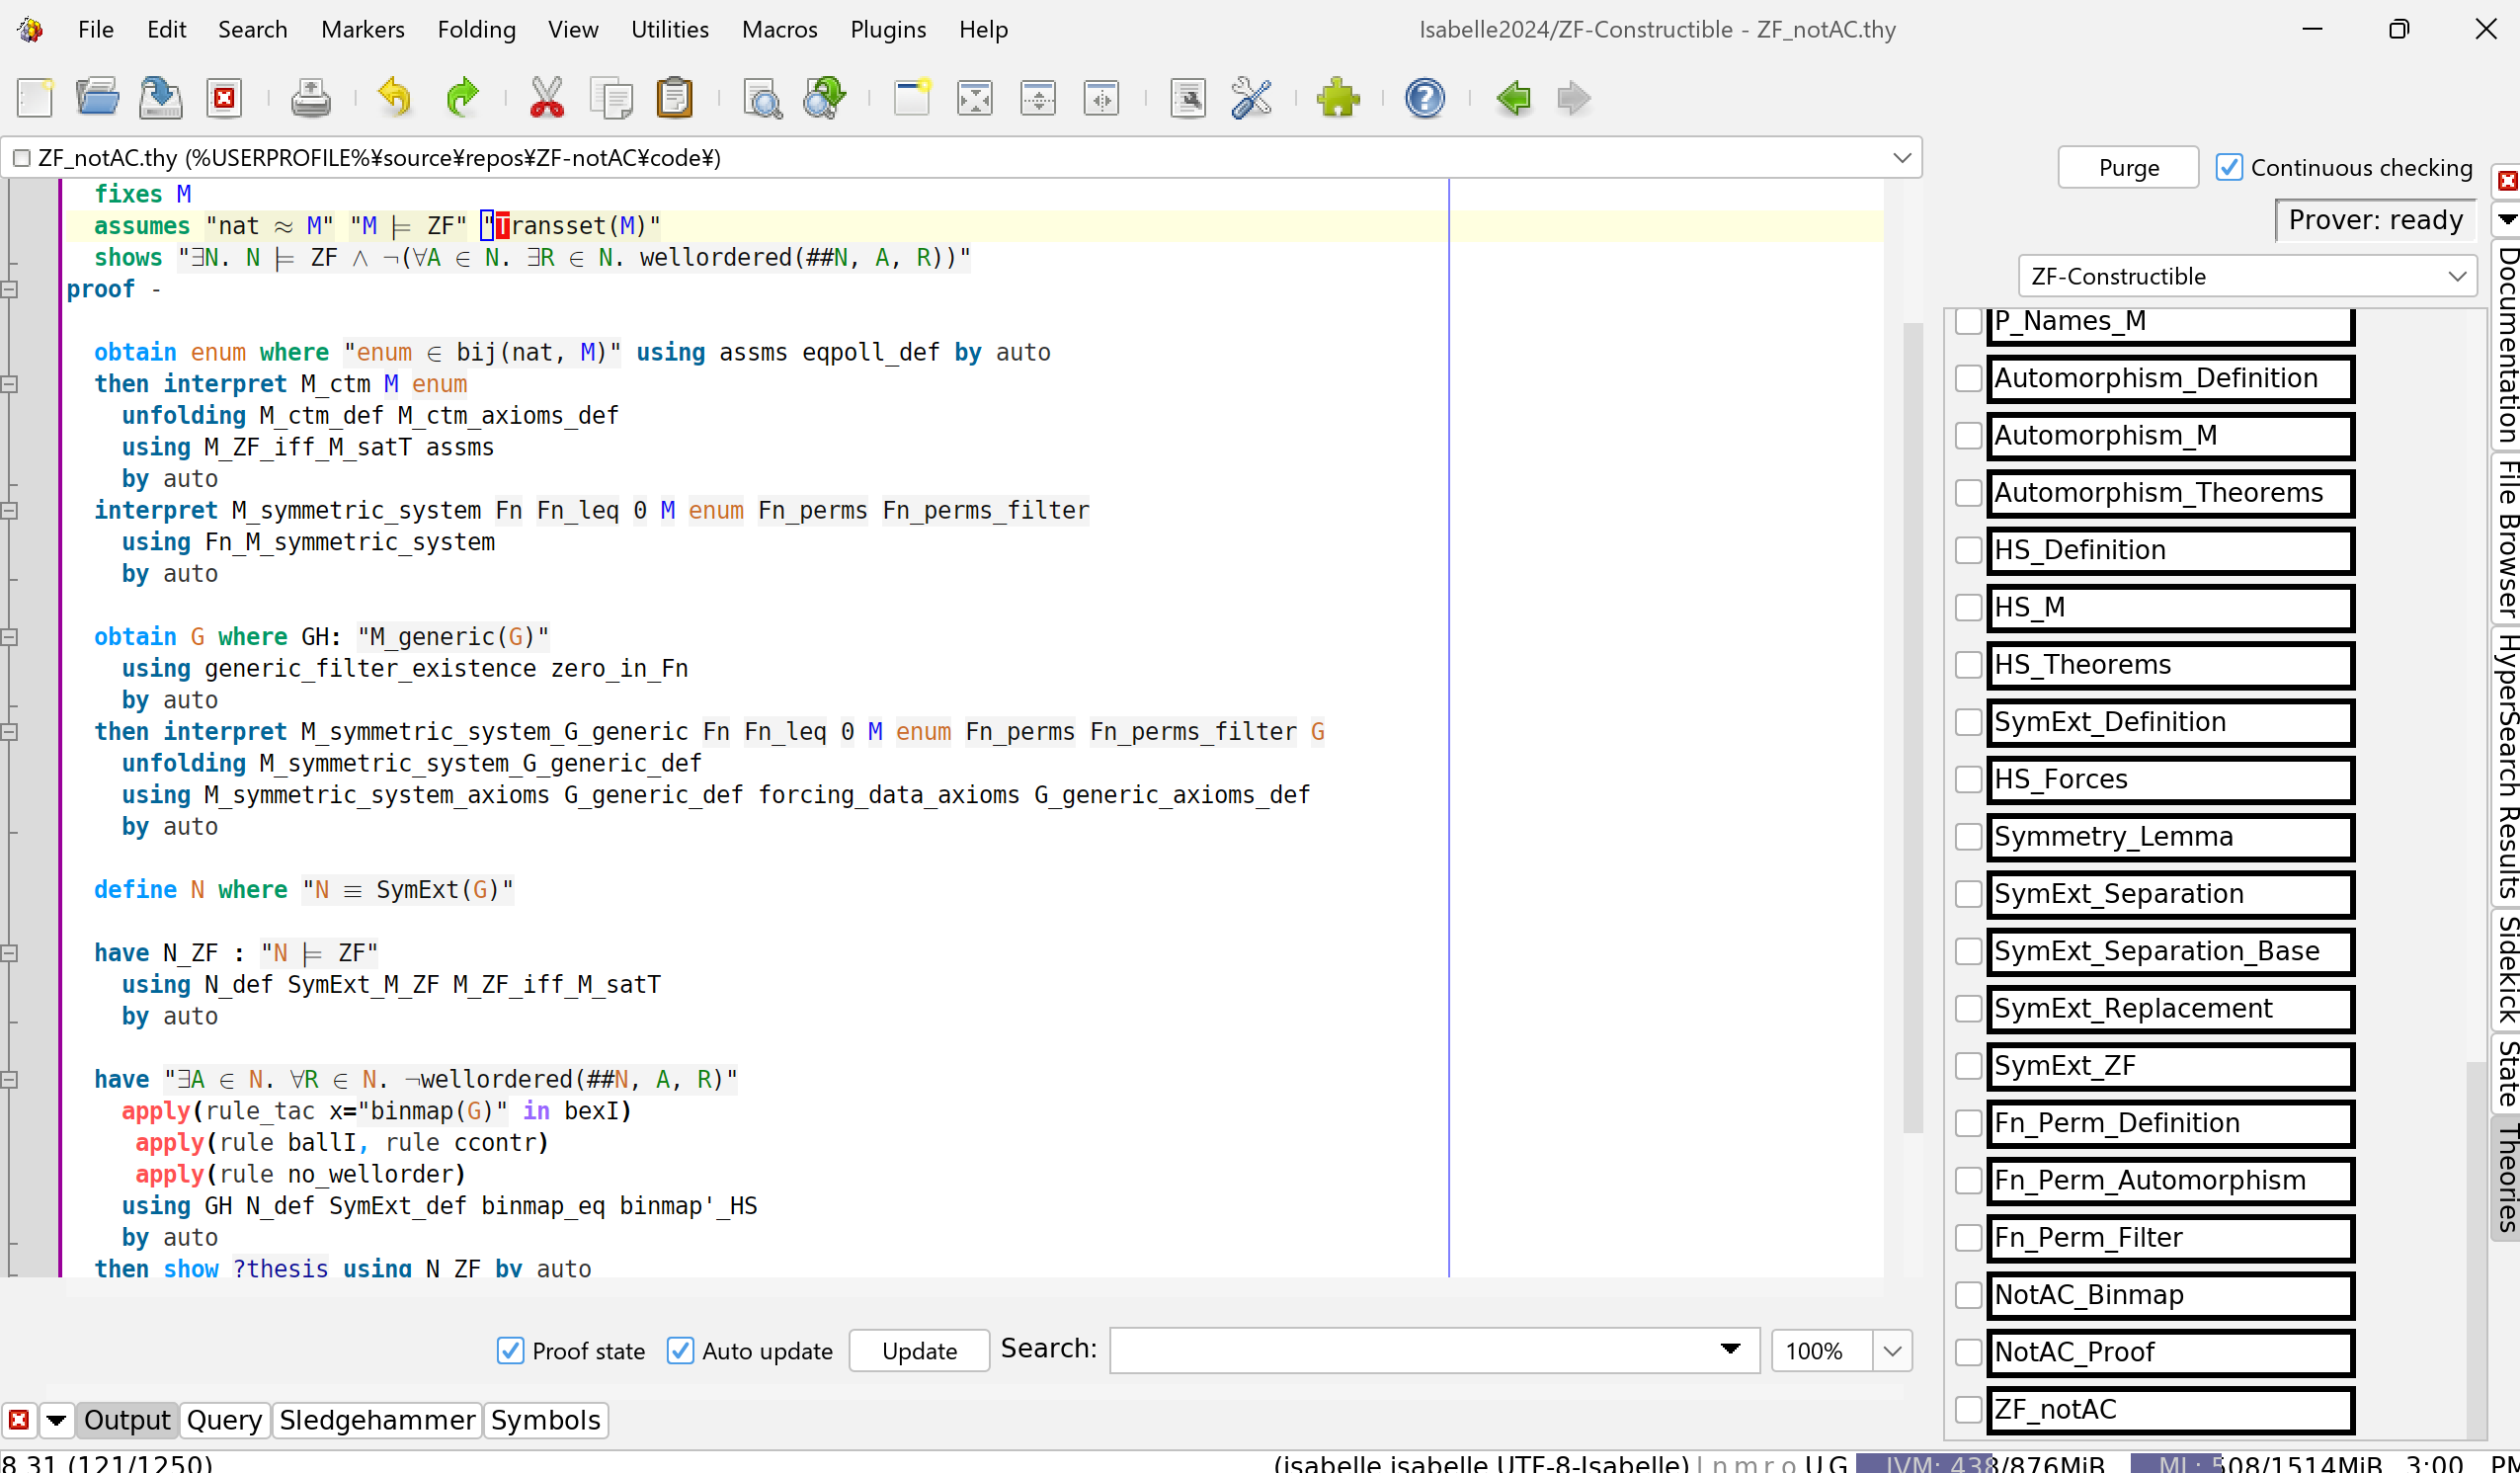
\includegraphics[width=1.0\linewidth]{./images/isabelle_editor.png}
            \end{figure}
            \vspace{-10pt}
            \begin{figure}
                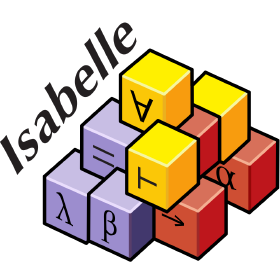
\includegraphics[width=0.7\linewidth]{./images/isabelle_logo.png}
            \end{figure}

        \end{column}
    \end{columns}

    %----------------------------------------------
    % coqの画像 https://ja.wikipedia.org/wiki/Coq#/media/%E3%83%95%E3%82%A1%E3%82%A4%E3%83%AB:CoqProofOfDecidablityOfEqualityOnNaturalNumbers.png
    %----------------------------------------------

\end{frame}

%----------------------------------------------
%    マイクロカーネル
%    https://read.seas.harvard.edu/~kohler/class/cs260r-17/klein10sel4.pdf
%----------------------------------------------

\begin{frame}{Isabelle {\small [Paulson 86]}}
    \vspace{-5pt}
    \begin{itemize}[itemsep=3pt]
        \item 実績
            \vspace{-3pt}
            \begin{itemize}[itemsep=2pt]
                \item seL4カーネルの形式検証 {\small \,[Klein et al. 14]}
                \item ALEXANDRIAプロジェクト{\small \,[Paulson 23]}
                \item ケプラー予想の形式証明{\small (の一部)[Hales et al. 15]}
                
            \end{itemize}
        \item Archive of Formal Proofs
    \end{itemize}
    
    \vspace{-10pt}
    \begin{columns}
        \begin{column}{0.25\textwidth}
            \vspace{-7pt}
            \begin{figure}
                
\includegraphics[width=0.9\linewidth]{./images/sel4-logo.png}
            \end{figure}
        \end{column}
        \begin{column}{0.33\textwidth}
            \vspace{-8pt}
            \begin{figure}
                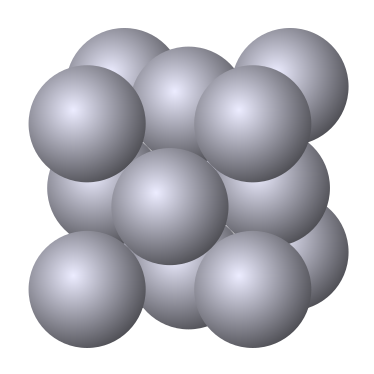
\includegraphics[width=0.6\linewidth]{./images/kepler2.png} %public domain
            \end{figure}
        \end{column}
        \begin{column}{0.35\textwidth}
            \vspace{-20pt} 
            \begin{figure}
                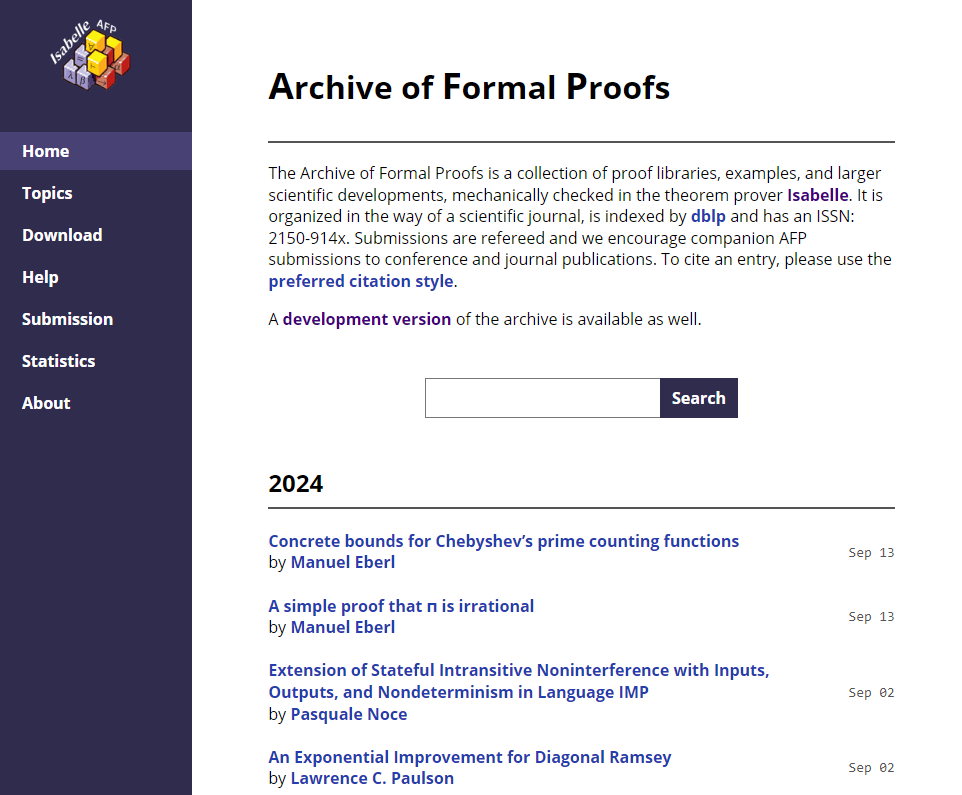
\includegraphics[width=0.8\linewidth]{./images/isabelle_archive.png}
            \end{figure}
        \end{column}
    \end{columns}
\end{frame}

\begin{frame}{Isabelle}
    \begin{itemize}
        \item 論理体系「Pure」上で定理証明を行う
        \item 「Pure」上に他の論理体系が構築されている
              {\small \begin{itemize}
                  \item Higher-Order Logic
                  \item First-Order Logic \\
                  \item \dots
              \end{itemize} }
              \vspace{-10pt}
        \item \textcolor{red}{Isabelle/ZF} $\cdots$ \\ 
        一階述語論理とZF(C)公理系のフレームワーク
    \end{itemize}
\end{frame}

% 簡単な定理証明の例を紹介するといいかも
% apply-script, structured proofの説明

% ZFの公理を記述しているコードを紹介するといいかも
% https://isabelle.in.tum.de/dist/library/FOL/ZF/ZF_Base.html ZFの公理のコード

\begin{frame}{Isabelle/ZFにおける先行研究}
 
    \begin{itemize}[itemsep=8pt]
        \vspace{10pt}
        \item CHのZFC上の独立性証明{\small [Gunther et al. 20,22]}
            \vspace{3pt}
              {\small \begin{itemize}
                \item 強制法の形式化 % 行数
                \item CHの独立性証明
              \end{itemize} }

        \item ACのZF上の相対的無矛盾性証明{\small [Paulson 02]}
              {\small \begin{itemize}
                      \item 構成可能宇宙を形式化
                  \end{itemize} }
              % https://arxiv.org/pdf/2001.09715 強制法の形式化
              % https://cs.famaf.unc.edu.ar/~pedro/forcing/Independence_CH/document.pdf CHの独立性証明
    \end{itemize}
    \begin{itemize}
        \item [\textcolor{red}{$\blacktriangleright$}] $\neg$ACの相対的無矛盾性証明は\\
        形式化されていなかったので挑戦
    \end{itemize}
\end{frame}

\begin{frame}{本研究におけるIsabelle/ZFの利点}
    \begin{itemize}
        \item 集合論に関する補題・糖衣構文が豊富
        \item Guntherらの強制法の形式化が使える
        {\small \begin{itemize}
            \item ZFのc.t.m.の存在を仮定している
            \begin{itemize}
                \item c.t.m. $\cdots$ countable transitive model
                \item この仮定により証明の形式化に\\ギャップが生じる(後述)
            \end{itemize}
        \end{itemize}}
    \end{itemize}
    ※本研究では相性の良いKaragila(2023)の証明に従う
\end{frame}


\section{証明概略}
\begin{frame}{証明概略}
    ZFのc.t.m. $M$から出発しZF+$\neg$ACのモデル$N$を構成
    \begin{itemize}[itemsep=8pt]
        \item あるposet $\mathbb{P}$によるgeneric extension $M[G]$の\\
              \textcolor{red}{symmetric extension}と呼ばれる\\
              部分モデル$N \subseteq M[G]$を構成
        \item $N$はZFを満たすが、整列可能定理を満たさない
    \end{itemize}
\end{frame}

\begin{frame}{symmetric extensionの定義(1)}
    \vspace{-5pt}
    \begin{itembox}[l]{定義 ($\Pbb$-name)}
        {\small
            \vspace{-5pt}
            MをZFのc.t.m.とする
            \vspace{-8pt}
            \begin{itemize}[itemsep=1pt]
                \item 最大元$1_{\Pbb}$をもつ疑順序集合$(\Pbb, \le_{\Pbb})$をposetという 
                \item $M^{\Pbb}_{\alpha}$を再帰的に定義する 
                    \begin{itemize}
                       \item $M^{\Pbb}_0 = \emptyset$ 
                       \item  $M^{\Pbb}_{\alpha+1} = \mathcal{P}^M(M^{\Pbb}_{\alpha} \times \Pbb)$ 
                       \item  $M^{\Pbb}_{\alpha} = \bigcup_{\beta < \alpha} M^{\Pbb}_{\beta}$\,\,\,\,($\alpha$はlimit ordinal)
                    \end{itemize}
                \item $M^{\Pbb} = \bigcup_{\alpha \in \text{Ord}} M^{\Pbb}_{\alpha}$とし、$M^{\Pbb}$の元を$\Pbb$-nameという
            \end{itemize}            
        }
    \end{itembox}
\end{frame}

\begin{comment}
    
\begin{frame}{symmetric extensionの定義(1)}
    \begin{itembox}[l]{定義 (自己同型)}
        {\small
            $(\Pbb, \le_{\Pbb})$は半順序で、最大元$1_{\Pbb}$をもつとする \\
            $\pi : \Pbb \rightarrow \Pbb$が自己同型であるとは次を満たすこと
            \begin{itemize}
                \setlength{\itemsep}{3pt}
                \item $\pi$は全単射
                \item $p, q \in \Pbb$に対して、$p \le_{\Pbb} q \Leftrightarrow \pi p \le_{\Pbb} \pi q$
            \end{itemize}
            $\pi$は以下のように$M^\Pbb$上の自己同型に拡張される
            $$ \pi \dot{x} = \{ (\pi \dot{y}, \pi p) | (\dot{y}, p) \in \dot{x} \} $$
        }
    \end{itembox}
\end{frame}

\end{comment}

\begin{frame}{symmetric extensionの定義(2)}
    \vspace{-7pt}
    \begin{itembox}[l]{定義(normal filter / {\small 自己同型の拡張})}
        {\small
            $\Gcal$を$\Pbb$の自己同型群とする  \\
            \textbullet\,\,\,$\Gcal$の部分群の族$\Fcal$がnormal filterであるとは次を満たすこと
            \vspace{-5pt}
            \begin{itemize}[left=1cm]
                \setlength{\itemsep}{0pt}
                \item [\textasteriskcentered] $H_1, H_2 \in \Fcal$に対して$H_1 \cap H_2 \in \Fcal$
                \item [\textasteriskcentered] super groupをとる操作で閉じている
                \item [\textasteriskcentered] $H \in \Fcal, \pi \in \Gcal$に対して$\pi H \pi^{-1} \in \Fcal$
            \end{itemize}
            \vspace{-3pt}
            \textbullet \,\,\,$\Pbb$の自己同型$\pi$を次のように$M^\Pbb$上の自己同型に拡張する
            \vspace{-5pt}
            $$ \pi \dot{x} = \{ (\pi \dot{y}, \pi p) | (\dot{y}, p) \in \dot{x} \} \text{ for } \dot{x} \in M^\Pbb $$
        }
            
    \end{itembox}
\end{frame}

\begin{frame}{symmetric extensionの定義(3)}
    \begin{itembox}[l]{定義 (hereditarily symmetric)}
        {\small
            $\Fcal$を$\Gcal$のnormal filterとする
            \vspace{5pt}
            \begin{itemize}
                \setlength{\itemsep}{2pt}
                \vspace{-10pt}
                \item $\dot{x} \in M^\Pbb$が$\Fcal$-symmetric $\Leftrightarrow \{ \pi \in \Gcal | \pi \dot{x} = \dot{x} \} \in \Fcal$
                \item $\dot{x}$がhereditarily $\Fcal$-symmetricとは以下を満たすこと
                      \vspace{-3pt}
                      \begin{itemize}
                          \item $\dot{x}$は$\Fcal$-symmetric
                          \item $\bm{\mathbf{dom}}(\dot{x})$の全ての要素はhereditarily $\Fcal$-symmetric
                      \end{itemize}
                \item hereditarily $\Fcal$-symmetricな$\dot{x}$の集合を$\bm{\mathbf{HS}}_{\Fcal}$とかく

            \end{itemize}
        }
    \end{itembox}
\end{frame}

\begin{frame}{symmetric extensionの定義(4)}
    \begin{itembox}[l]{定義 (symmetric extension)}
        {\small
            $\Pbb$-generic filter $G$に対し、\\$\{ \dot{x}_G | \dot{x} \in \bm{\mathbf{HS}}_{\Fcal} \}$をsymmetric extensionという
        }
    \end{itembox}

    \begin{itemize}
        \item symmetric extensionは、ZFのモデルとなる
    \end{itemize}
\end{frame}

\section {Isabelle/ZFによる形式化}

\begin{frame}{成果}
    本研究で証明した主定理
    \vspace{-1cm}
    \hspace{-1.5cm}
    \begin{figure}
        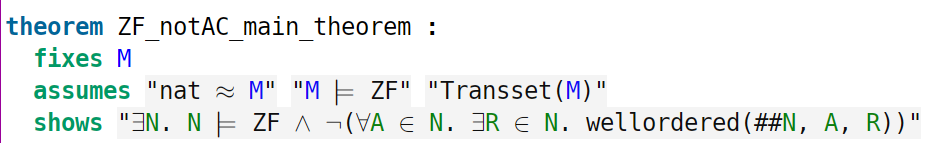
\includegraphics[width=1.1\linewidth]{./images/ZF_notAC_main_theorem.png}
    \end{figure}

    \vspace{-5pt}
    意味 \\
    {\small
    \hspace{1cm} $M$をZFのc.t.m.とする。このとき、ある$N$があって、\\
    \hspace{1cm} $N$はZFを満たすが、整列可能定理を満たさない
    }
\end{frame}

\begin{frame}{作業工程}
    以下の工程に分けられる
    {\small
    \begin{itemize}[itemsep=8pt]
        \item symmetric extensionの定義
        \item ZFのモデルであることの証明
        \item 特定のsymmetric extensionの構成
        \item それが$\neg$ACを満たすことの証明
    \end{itemize} }
\end{frame}

\begin{frame}{作業量}
    \makebox[\textwidth]{約1万5千行のコード \hfill {\small 補題など(3千行)}}
    {\small
        \begin{itemize}[itemsep=8pt]
            \item symmetric extensionの定義(3千行)
            \item ZFのモデルであることの証明(5千行)
            \item 特定のsymmetric extensionの構成(2千行)
            \item それが$\neg$ACを満たすことの証明(2千行)
        \end{itemize} }
\end{frame}

\begin{frame}{苦労した点\, {\normalsize 1.自明なことの確認}}

    「自明なこと」の確認が非常に大変な場合がある

    {\small
    \begin{itemize}
        \item 定義した関数が「本当に関数であること」
        \item クラスに「本当にそれを表す論理式が存在すること」
    \end{itemize}
    }
\end{frame}

\begin{frame}{苦労した点\, {\normalsize 1.自明なことの確認}}
    特に、「帰納的に定義された$M$内の関数」の場合

    {\small
    \begin{itemize}
        \item そもそも「$M$の元であること」の確認も必要
              {\footnotesize
              \begin{itemize}
                  \item 仮定とZFの公理からちゃんと構成できるか?
              \end{itemize}}
        \item このような関数を定義するための補題が2千行以上
    \end{itemize}
    }
\end{frame}

\begin{frame}{苦労した点\, {\normalsize 2.先行研究の定義}}
    先行研究の強制関係の定義
    {\small
    \begin{itemize}[itemsep=8pt]
        \item よくあるfor allに対する強制関係の定義
              $$ p \Vdash \forall x \phi(x, \dot{x_1}, ..., \dot{x_n}) \Leftrightarrow \forall \dot{x} \in M^\Pbb(p \Vdash \phi(\dot{x}, \dot{x_1}, ..., \dot{x_n})) $$
        \item 先行研究の定義
              $$ p \Vdash \forall x \phi(x, \dot{x_1}, ..., \dot{x_n}) \Leftrightarrow \forall x \in \textcolor{red}{M}(p \Vdash \phi(x, \dot{x_1}, ..., \dot{x_n})) $$
    \end{itemize}
    \vspace{-6pt}
    \hspace{1cm}※この定義でうまくいくように他の部分も修正されている
    }
\end{frame}

\begin{frame}{苦労した点\, {\normalsize 2.先行研究の定義}}
    帰納法に$\Pbb$-nameでないものが混入する...
    {
    \small
    \begin{itemize}[itemsep=8pt]
        \item $\mathbf{val}(G, \cdot)$を$M$上の関数として定義している
              $$\mathbf{val}(G, x) := \{ \mathbf{val}(G, y) | y \in \mathbf{dom}(x), \exists p \in G. (y, p) \in x \}$$
        \item $x \in M$に対しある$\dot{z} \in M^\Pbb$があって$\mathbf{val}(x, G) = \mathbf{val}(\dot{z}, G)$
              \vspace{5pt}
              \begin{itemize}
                  \item この事実を形式化して一度は困難を解決
                  \item 最終的には別手法で「苦労した点3.」と同時に解決
              \end{itemize}
    \end{itemize}

    }
\end{frame}

\begin{frame}{苦労した点\, {\normalsize 3.ZFのモデルであることの証明}}
    symmetric extensionがZFのモデルであることの証明
    \begin{itembox}[l]{命題}
        {\small
            $N$が推移的かつalmost universalなクラスで、$\Delta_0$-separationを\\
            満たすならば、$N$はZFの内部モデルである
        }
    \end{itembox}
    {\small
    \begin{itemize}[itemsep=8pt]
        \item 参考資料ではこの命題を証明に用いている
        \item 前提条件は証明できたが、「命題自体」が証明できなかった
    \end{itemize}
    }
\end{frame}

\begin{frame}{苦労した点\, {\normalsize 3.ZFのモデルであることの証明}}

    \begin{itembox}[l]{命題(Collection Principle, Jech「Set Theory」6.5)}
        {\small $p$をパラメータとして}
        \vspace{-10pt}
        $$\forall X \exists Y (\forall u \in X)[\exists v \phi(u, v, p) \rightarrow (\exists v \in Y) \phi(u, v, p)]$$
    \end{itembox}

    \vspace{-5pt}
    {\small
        \begin{itemize}[itemsep=5pt]
            \item 具体的にはこの命題の証明で行き詰った
            \item symmetric extensionが、generic extensionで\\
                  definebleなクラスであることが証明できなかった
        \end{itemize}
    }

\end{frame}

\begin{frame}{苦労した点\, {\normalsize 3.ZFのモデルであることの証明}}
    代替手段
    \vspace{-10pt}
    {\small
        \begin{itemize}[itemsep=8pt]
            \item HSに相対化した強制関係$\textcolor{red}{\Vdash_{\mathbf{HS}}}$を形式化
                  \begin{itemize}
                      \item 参考資料に書かれている概念
                      \item 強制関係の定義の量化の動く範囲を$\mathbf{HS}$に制限
                      \item $\Vdash_{\mathbf{HS}}$は、symmetric extensionに対し、\\
                            generic extensionに対する$\Vdash$のように振舞う
                  \end{itemize}
            \item $\Vdash_{\mathbf{HS}}$を用いてZFのモデルであることを証明
                  \begin{itemize}
                      \item 強制関係の帰納法が不要になり{\footnotesize「苦労した点2.」}も解決
                  \end{itemize}
        \end{itemize}
    }
\end{frame}


\section {まとめ}

\begin{frame}{まとめ}
    $\neg$ACの相対的無矛盾性証明をIsabelle/ZFで形式化
    {\small
    \begin{itemize}[itemsep=8pt]
        \item ZFのc.t.m.から出発し、\\ZF+$\neg$ACをみたすsymmetric extensionを構成
        \item 厳密な意味での相対的無矛盾性の証明とはギャップがある
        \item 参考資料の通りにいかず試行錯誤した部分も
        \item 先行研究の改善点を発見?
    \end{itemize}
    }
\end{frame}

\appendix
\setbeamertemplate{footline}{}

\begin{frame}{ギャップ}
    \vspace{-15pt}
    \,
    {\small 
    \begin{itemize}[itemsep=5pt]
        \item 既存のIsabelle/ZFでの強制法の形式化は\\ZFのc.t.m.の存在を仮定したもの
        \item これを用いるため、\\本研究でもZFのc.t.m.を仮定する
        \item ZFのc.t.m.の存在は、Con(ZF)から証明できない
        \item 本当の意味での相対的無矛盾性Con(ZF) $\rightarrow$ Con(ZF+$\neg$AC)\\
        の証明とはギャップがある
    \end{itemize}
    }
\end{frame}

\begin{frame}{ギャップ}
    c.t.m.を用いた議論の背景
\end{frame}

\begin{frame}{ギャップ}
    \begin{itemize} 
        \item Boolean-valued modelなど\\
              別のアプローチをとれなかったのか?
        \item 強制法の形式化部分で\\作業量が増えてしまうので断念
    \end{itemize}    
\end{frame}


\end{document}


